

\capitulo{5}{Resultados}

\section{Resumen de resultados.}
El presente proyecto presenta un prototipo hardware/software funcional, el cual tiene un gran potencial para servir como ayuda tanto al paciente con párkinson como al profesional sanitario. Provee al paciente una ayuda visual en tiempo real para superar rápidamente y de mejor manera los congelamientos de la marcha, los cuales se detectan de forma personalizada para adecuarse a las características del usuario. También proporciona avances en el análisis de la evolución de la enfermedad, permitiendo descargar informes con los datos recogidos, visualizar gráficas sobre dichos datos y tener en cuenta la percepción del paciente sobre sus fluctuaciones motoras.

El trabajo realizado ha completado los objetivos hardware propuestos en cuanto a la creación de un nuevo prototipo incluyendo un módulo láser y diseñado dicho hardware de forma más cómoda que en previos prototipos, insertando los componentes en un cinturón y una tobillera, como se muestra en las imágenes \ref{fig:prototipo} \ref{fig:prototipoencendido}.

\begin{figure}[h]
    \centering
    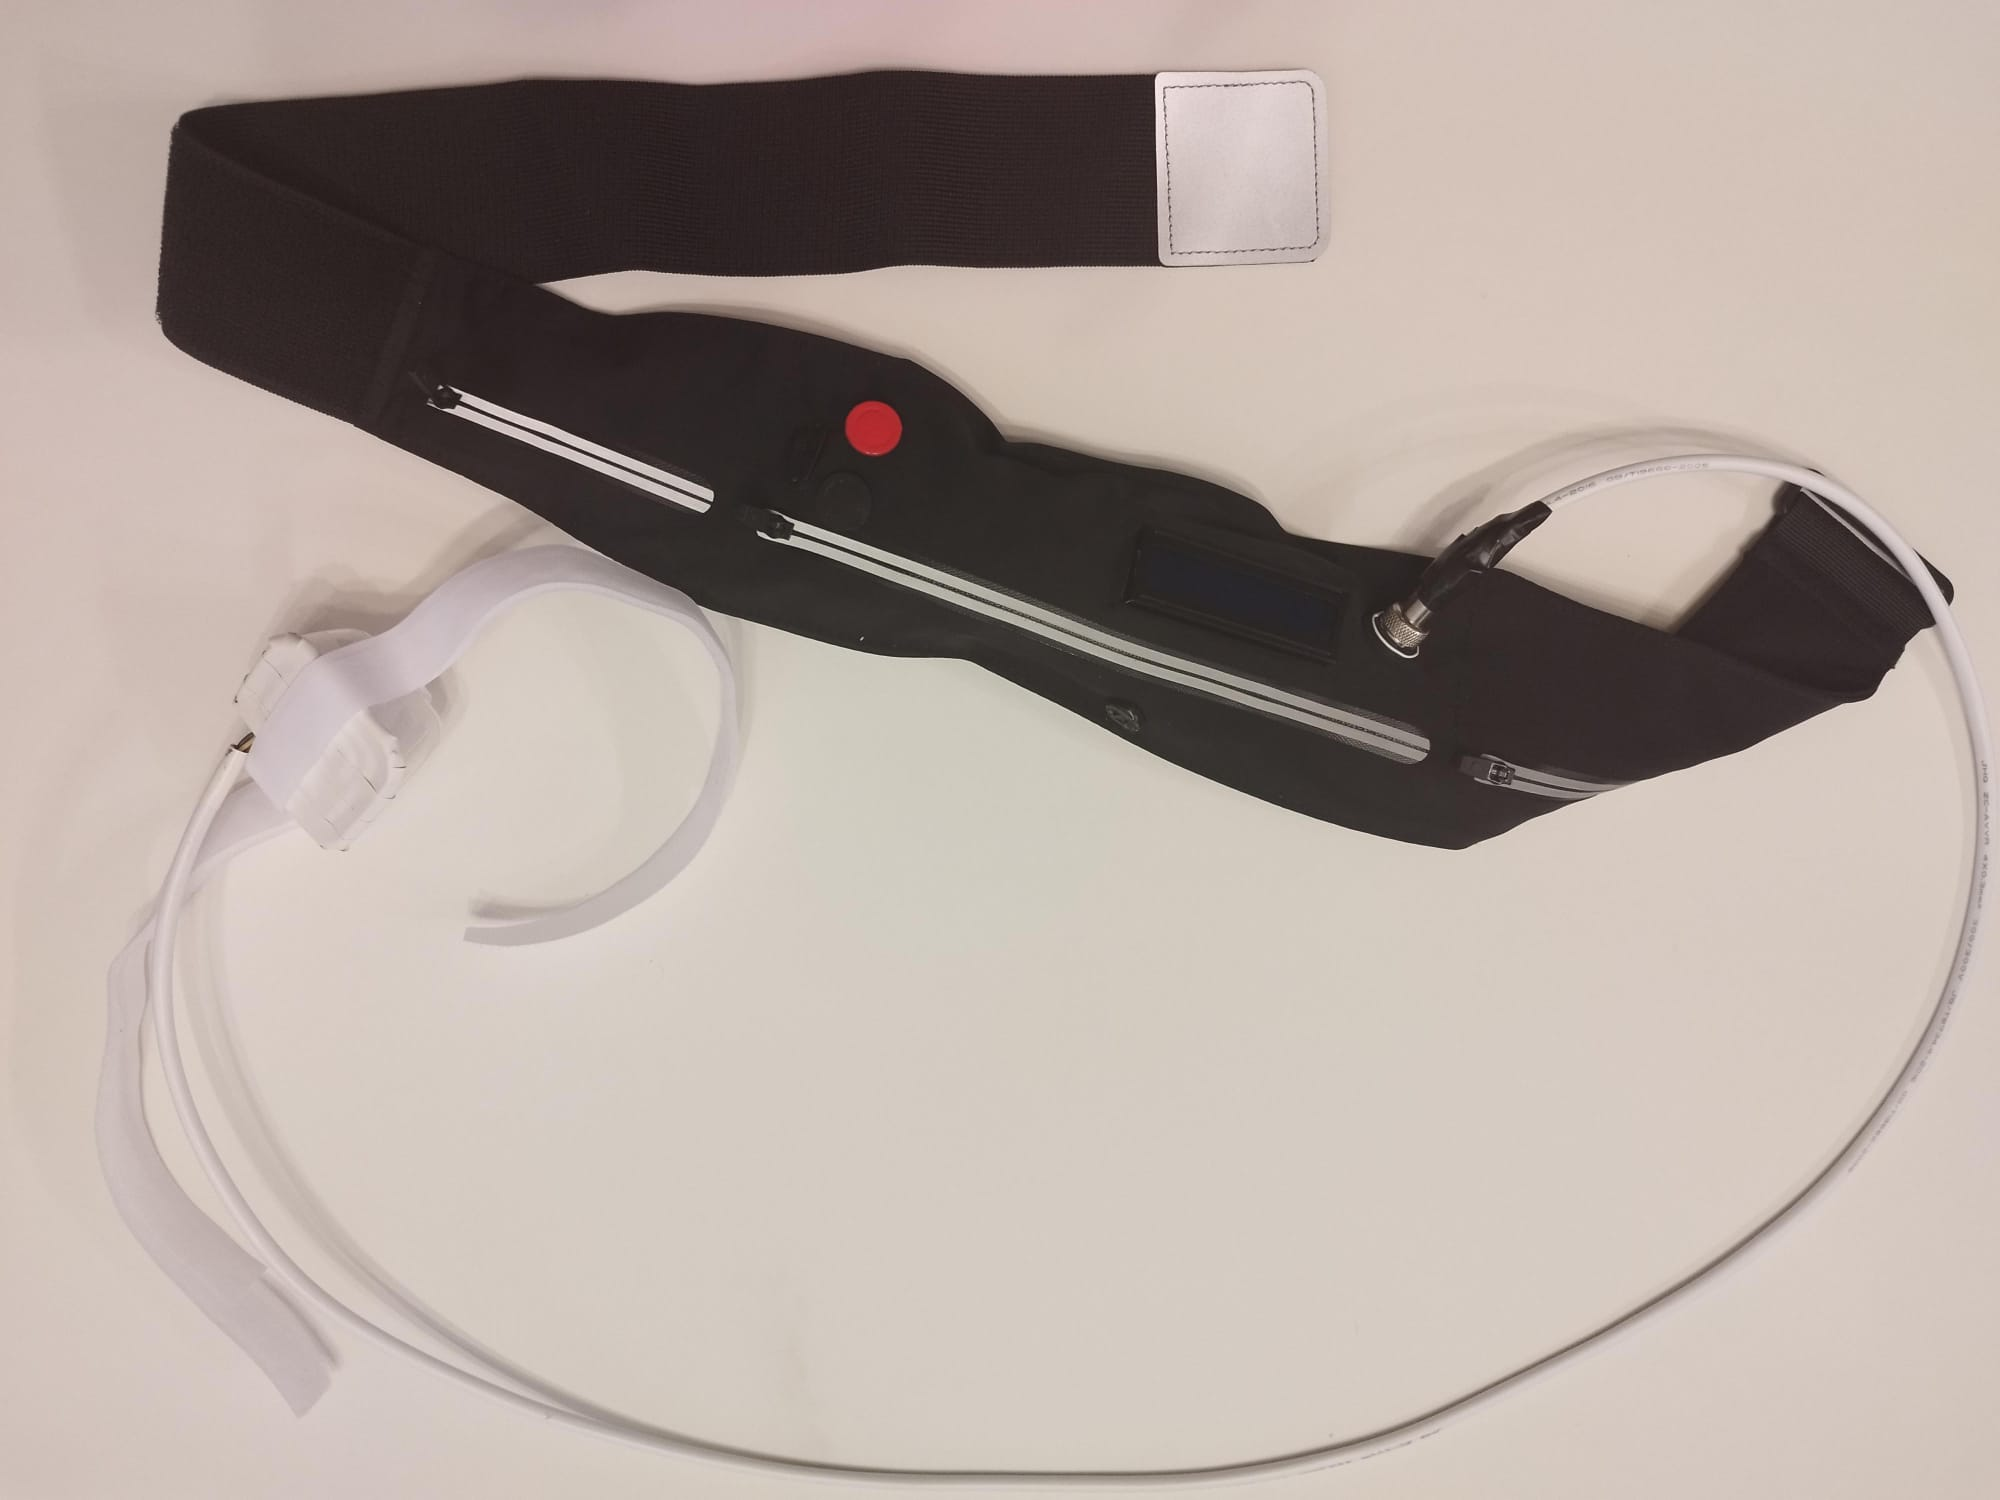
\includegraphics[width=1\textwidth]{img/prototipocompleto.jpg}
    \caption{Prototipo hardware completo. Fuente propia.}
    \label{fig:prototipo}
\end{figure}

\begin{figure}[h]
    \centering
    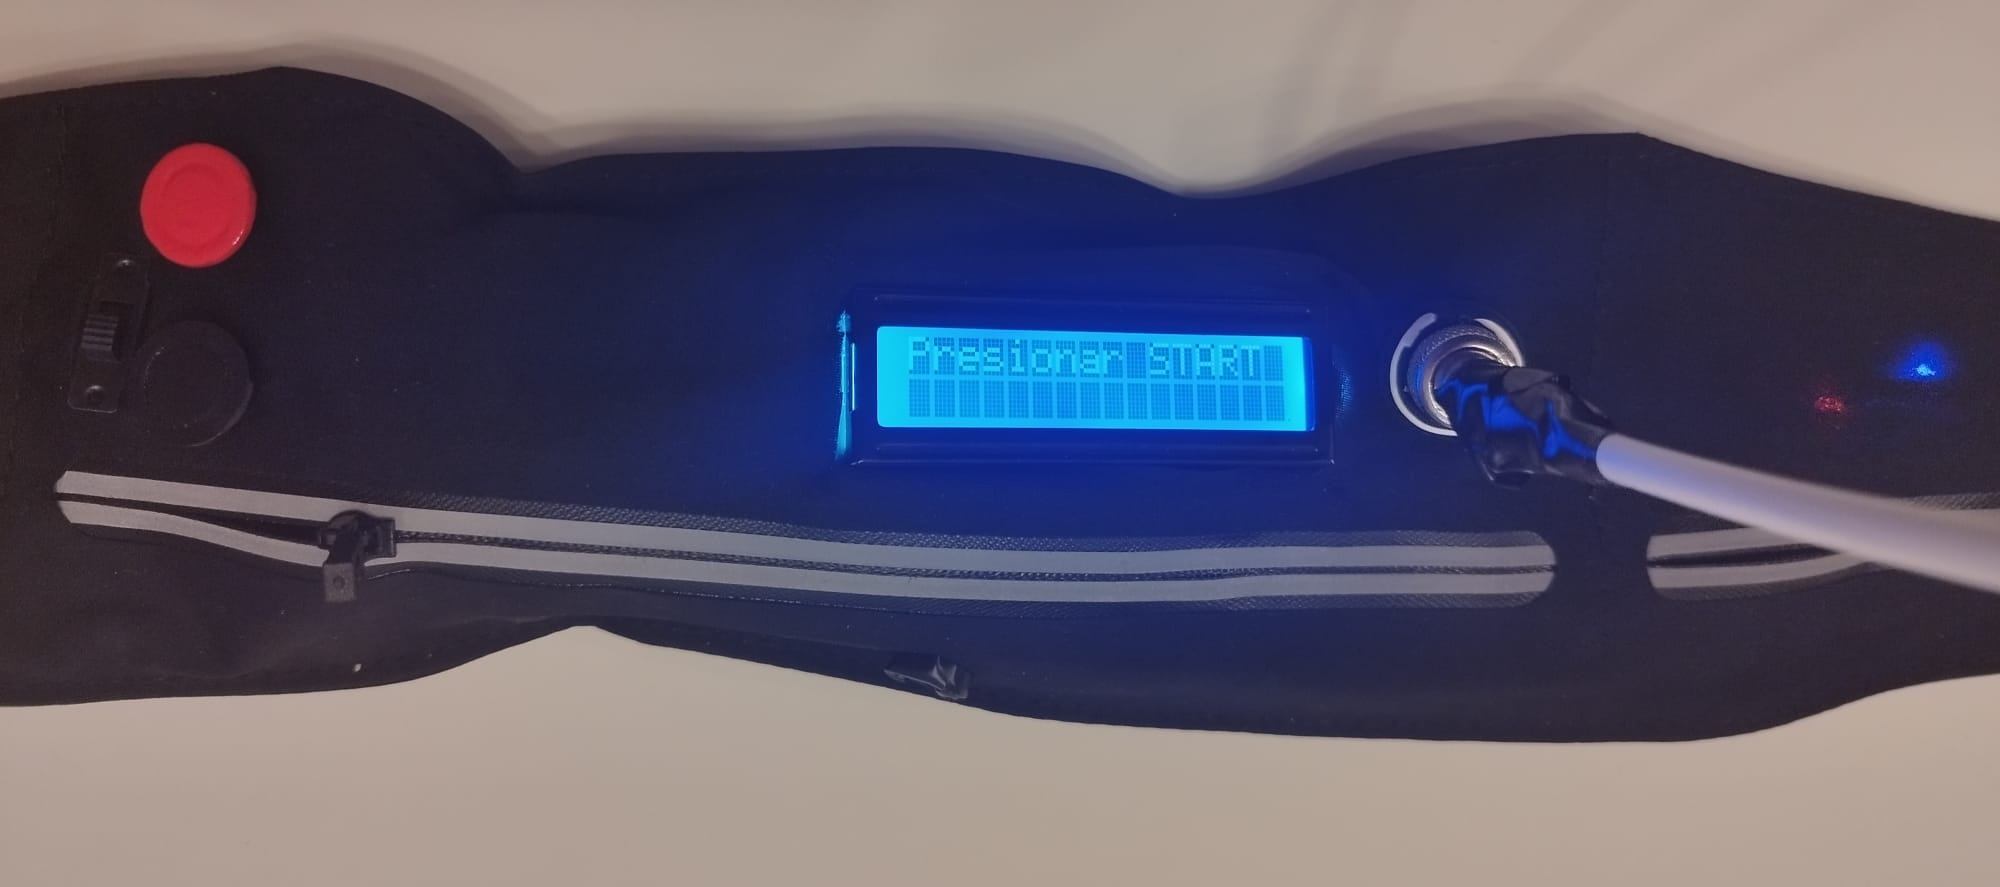
\includegraphics[width=1\textwidth]{img/prototipoencendido.jpg}
    \caption{Prototipo hardware encendido. Fuente propia.}
    \label{fig:prototipoencendido}
\end{figure}

Se alcanzaron los objetivos software relativos a la aplicación web: función de inserción de pautas de medicación para un paciente por parte de usuarios de tipo 'profesional', función web para los usuarios de tipo 'paciente' de registro de un diario de tomas de medicaciones y fluctuaciones motoras, prueba de personalización del número de segundos que el dispositivo detecta como congelamiento muscular, generación de gráficas a partir de los datos registrados y descarga de un informe relativo a las actividades registradas.

El script de Arduino fue editado satisfactoriamente, flexibilizando la detección de congelamientos de la marcha para tener en cuenta la prueba de personalización y controlando el encendido de módulo láser al detectar dichos congelamientos.

El objetivo relativo al almacenamiento de fecha y hora de cada actividad mediante implementación de un módulo de reloj RTC en el hardware fue alcanzado con un método distinto: almacenando la fecha y hora de guardado de cada actividad utilizando javascript, sin adición de módulos software adicionales.
\section{Discusión.}
Con el objetivo de contextualizar los resultados obtenidos durante el proyecto, se presenta una comparación de las características más relevantes de los mismos con los resultados otros trabajos.

En la tabla \ref{tab:comparacion1} se comparan las funciones de la solución tecnológica presentada en el artículo \cite{GONCALVES2021115653}, el cual ha sido previamente analizado en el apartado 'Conceptos teóricos' de este trabajo. Esta solución tecnológica ha sido escogida para realizar esta comparación debido a las inmensas similitudes en ambos proyectos: utilización de sensor inercial MPU-6050 para la monitorización de la marcha en pacientes con Párkinson, desarrollo de aplicación móvil conectada al hardware... 

% Please add the following required packages to your document preamble:
% \usepackage[table,xcdraw]{xcolor}
% Beamer presentation requires \usepackage{colortbl} instead of \usepackage[table,xcdraw]{xcolor}
\begin{table}[]
\begin{tabular}{l|
>{\columncolor[HTML]{FFFFFF}}l |
>{\columncolor[HTML]{FFFFFF}}l |}
\cline{2-3}
                                                                                                                                                                              & \cellcolor[HTML]{C0C0C0}Proyecto actual & \cellcolor[HTML]{C0C0C0}\begin{tabular}[c]{@{}l@{}}Sistema de \\monitorización\\ de la marcha\end{tabular} \\ \hline
\multicolumn{1}{|l|}{\cellcolor[HTML]{EFEFEF}\begin{tabular}[c]{@{}l@{}}Adquisición de datos \\ con MPU-6050\end{tabular}}                                                    & Sí                                      & Sí                                                                                                       \\ \hline
\multicolumn{1}{|l|}{\cellcolor[HTML]{EFEFEF}\begin{tabular}[c]{@{}l@{}}Unidad de almacenamiento \\ de datos (tarjeta SD)\end{tabular}}                                       & No                                      & Sí                                                                                                       \\ \hline
\multicolumn{1}{|l|}{\cellcolor[HTML]{EFEFEF}\begin{tabular}[c]{@{}l@{}}Comunicación bluetooth \\ con aplicación móvil\end{tabular}}                                          & Sí                                      & Sí                                                                                                       \\ \hline
\multicolumn{1}{|l|}{\cellcolor[HTML]{EFEFEF}\begin{tabular}[c]{@{}l@{}}Transmisión de los datos obtenidos\\  en tiempo real a la app\end{tabular}}                           & Sí                                      & Sí                                                                                                       \\ \hline
\multicolumn{1}{|l|}{\cellcolor[HTML]{EFEFEF}\begin{tabular}[c]{@{}l@{}}Integración de los datos con un \\ diario de síntomas del paciente\end{tabular}}                      & Sí                                      & No                                                                                                       \\ \hline
\multicolumn{1}{|l|}{\cellcolor[HTML]{EFEFEF}Generación de gráficas con los datos}                                                                                            & Sí (más básicas)                        & Sí                                                                                                       \\ \hline
\multicolumn{1}{|l|}{\cellcolor[HTML]{EFEFEF}Generación de informes pdf}                                                                                                      & Sí                                      & No                                                                                                       \\ \hline
\multicolumn{1}{|l|}{\cellcolor[HTML]{EFEFEF}\begin{tabular}[c]{@{}l@{}}Interfaz de escritorio en MATLAB para \\ el análisis detallado de los datos almacenados\end{tabular}} & No                                      & Sí                                                                                                       \\ \hline
\end{tabular}
\caption{Comparación entre el presente proyecto y un proyecto externo analizado previamente \cite{GONCALVES2021115653} }
\label{tab:comparacion1}
\end{table}

Teniendo en cuenta que el presente trabajo propone mejoras sobre un prototipo previamente construido a lo largo de los proyectos \cite{Gonzalez2023} \cite{Martos2024}  es importante diferenciar los aspectos del prototipo final que ya habían sido alcanzados en proyectos previos de las novedades. Esta diferencia puede observarse en la tabla \ref{tab:comparacion2}.
% Please add the following required packages to your document preamble:
% \usepackage[table,xcdraw]{xcolor}
% Beamer presentation requires \usepackage{colortbl} instead of \usepackage[table,xcdraw]{xcolor}
\begin{table}[]
\begin{tabular}{l|
>{\columncolor[HTML]{FFFFFF}}l |
>{\columncolor[HTML]{FFFFFF}}l |}
\cline{2-3}
                                                                                                                                                                                                 & \cellcolor[HTML]{C0C0C0}Proyecto actual & \cellcolor[HTML]{C0C0C0}Prototipos anteriores \\ \hline
\multicolumn{1}{|l|}{\cellcolor[HTML]{EFEFEF}\begin{tabular}[c]{@{}l@{}}Adquisición de datos \\ con MPU-6050\end{tabular}}                                                                       & Sí                                      & Sí                                            \\ \hline
\multicolumn{1}{|l|}{\cellcolor[HTML]{EFEFEF}\begin{tabular}[c]{@{}l@{}}Comunicación bluetooth \\ con aplicación móvil\end{tabular}}                                                             & Sí                                      & Sí                                            \\ \hline
\multicolumn{1}{|l|}{\cellcolor[HTML]{EFEFEF}\begin{tabular}[c]{@{}l@{}}Transmisión de los datos obtenidos\\  en tiempo real a la app\end{tabular}}                                              & Sí                                      & Sí                                            \\ \hline
\multicolumn{1}{|l|}{\cellcolor[HTML]{EFEFEF}\begin{tabular}[c]{@{}l@{}}Almacenamiento de los datos en base\\ de datos SQL\end{tabular}}                                                         & Sí                                      & Sí                                            \\ \hline
\multicolumn{1}{|l|}{\cellcolor[HTML]{EFEFEF}\begin{tabular}[c]{@{}l@{}}Recogida de datos diarios sobre\\ fluctuaciones motoras y tomas\\ de medicación\end{tabular}}                            & Sí                                      & No                                            \\ \hline
\multicolumn{1}{|l|}{\cellcolor[HTML]{EFEFEF}\begin{tabular}[c]{@{}l@{}}Integración de los datos con un \\ diario de síntomas del paciente\end{tabular}}                                         & Sí                                      & No                                            \\ \hline
\multicolumn{1}{|l|}{\cellcolor[HTML]{EFEFEF}Generación de gráficas con los datos}                                                                                                               & Sí (básicas)                            & No                                            \\ \hline
\multicolumn{1}{|l|}{\cellcolor[HTML]{EFEFEF}Generación de informes pdf}                                                                                                                         & Sí                                      & No                                            \\ \hline
\multicolumn{1}{|l|}{\cellcolor[HTML]{EFEFEF}\begin{tabular}[c]{@{}l@{}}Personalización del tiempo de reposo del \\ sensor MPU-6050 que se considera \\ congelamiento de la marcha\end{tabular}} & Sí                                      & No                                            \\ \hline
\end{tabular}
\caption{Comparación entre el presente proyecto y prototipos anteriores }
\label{tab:comparacion2}
\end{table}

